
%%%%%%%%%%%%%%%%%%%%%%%%%%%%%%%%%%%%%%%%%%%%%%%%%%%%%%%%%%%%
\subsubsection{Vertical component magnetic field ($\mathbf{b_z}$)}\label{section_bz}
After identifying the position of the source, assuming it is a dipole, we can utilize the modified approach from \citet{Oliveira2015Estimation} to calculate the dipole moment vector, denoted as 
\textbf{m}. The magnetic induction vector $\mathbf{b_z}$ for a dipole is given by

\begin{equation}
\label{eq_dipole_bz}
\mathbf{b_z}
= \dfrac{\mu_0}{4\pi}
\begin{bmatrix}
\dfrac{\partial^2}{\partial z \partial x} \dfrac{1}{r}
& \dfrac{\partial^2}{\partial z \partial y} \dfrac{1}{r}
& \dfrac{\partial^2}{\partial z \partial z} \dfrac{1}{r}
\end{bmatrix}
\begin{bmatrix}
m_x \\ m_y \\ m_z
\end{bmatrix}
= \dfrac{\mu_0}{4\pi} \mathbf{M_z}\,\mathbf{m}
\ .
\end{equation}

To address the mutual interference of magnetic sources, a method involves simultaneously solving the magnetic moment inversion for all "L" identified, therefore the Equation \ref{eq_dipole_bz} becomes


\begin{equation}
% \footnotesize
\label{eq_dipole_bz_all}
\dfrac{\mu_0}{4\pi}
{\begin{bmatrix}
\dfrac{\partial^2}{\partial z \partial x} \dfrac{1}{r_{1,1}}
& \dfrac{\partial^2}{\partial z \partial y} \dfrac{1}{r_{1,1}}
& \dfrac{\partial^2}{\partial z \partial z} \dfrac{1}{r_{1,1}}
& \hdots
& \dfrac{\partial^2}{\partial z \partial x} \dfrac{1}{r_{1,L}}
& \dfrac{\partial^2}{\partial z \partial y} \dfrac{1}{r_{1,L}}
& \dfrac{\partial^2}{\partial z \partial z} \dfrac{1}{r_{1,L}} \\
\\

& 
& 
& \vdots
& 
& 
&  \\
\\
\dfrac{\partial^2}{\partial z \partial x} \dfrac{1}{r_{N,1}}
& \dfrac{\partial^2}{\partial z \partial y} \dfrac{1}{r_{N,1}}
& \dfrac{\partial^2}{\partial z \partial z} \dfrac{1}{r_{N,1}}
& \hdots
& \dfrac{\partial^2}{\partial z \partial x} \dfrac{1}{r_{N,L}}
& \dfrac{\partial^2}{\partial z \partial y} \dfrac{1}{r_{N,L}}
& \dfrac{\partial^2}{\partial z \partial z} \dfrac{1}{r_{N,L}} \\
\end{bmatrix}}_{N \times 3L}
{\begin{bmatrix}
{m_x}_1 \\ {m_y}_1 \\ {m_z}_1 \\ \vdots \\{m_x}_L \\ {m_y}_L \\ {m_z}_L \\
\end{bmatrix}}_{3L \times 1}
=
{\begin{bmatrix}
{b_z}_1 \\ {b_z}_2 \\ {b_z}_3 \\ \vdots \\{b_z}_N 
\end{bmatrix}}_{N \times 1}.
\end{equation} \bigskip

In which $r_{i,j} = \sqrt{(x_i - {x_c}_j)^2 + (y_i - {y_c}_j)^2 + (z_i - {z_c}_j)^2}$ is the Cartesian distance between the i-th, $i=1, 2, \hdots N$, observation point $b_z (x_i, y_i, z_i)$ and the j-th, $j=1, 2, \hdots L$, point source $({x_c}_j, {y_c}_j, {z_c}_j)$ and $\mu_0$ is the vacuum magnetic permeability. While the three second-order derivatives in Equation~\ref{eq_dipole_bz_all} are:

\begin{equation}
% \footnotesize
\begin{aligned}
\dfrac{\partial^2}{\partial z \partial x} \dfrac{1}{r_{i,j}} &=
\dfrac{3(z_i - {z_c}_j)(x_i - {x_c}_j)}{{r_{i,j}}^5}\ ,
\\
\dfrac{\partial^2}{\partial z \partial y} \dfrac{1}{r_{i,j}} &=
\dfrac{3(z_i - {z_c}_j)(y_i - {y_c}_j)}{{r_{i,j}}^5}\ ,
\\
\dfrac{\partial^2}{\partial z \partial z} \dfrac{1}{r_{i,j}} &=
\dfrac{3(z_i - {z_c}_j)^2}{{r_{i,j}}^5} - \dfrac{1}{{r_{i,j}}^3}\ .
\end{aligned}
\end{equation}   \bigskip

The Equation \ref{eq_dipole_bz_all} can be expressed in matrix form as

\begin{equation}
\label{qdhqM4s9Ln}
\mathbf{M_z} \mathbf{m} = \mathbf{b_z}^{pred} \ .
\end{equation}

The dipole moment vector that best fits
a set of $N$ observations of the vertical component of the magnetic field
$\mathbf{b_z}^{obs}$ is given by minimizing the misfit function using a least-squares estimator

\begin{equation}
\label{uV9pRVYO4l}
\Phi (\mathbf{m}) = \| \mathbf{b_z}^{obs} - \mathbf{b_z}^{pred} \|^2 = (\mathbf{b_z}^{obs} - \mathbf{M_z}\mathbf{m})^T  (\mathbf{b_z}^{obs} - \mathbf{M_z}\mathbf{m})\ .
\end{equation}

The dipole moment vector that minimizes $\Phi (\mathbf{m})$ can be found by solving the linear equation system

\begin{equation}
 \mathbf{m} = {\left ( \mathbf{M_z}^T \mathbf{M_z} \right )}^{-1} \mathbf{M_z}^T\mathbf{b_z}^{obs}\ .
\end{equation}

Therefore, taking into account all their mutual signal interference in the N observed data increases further the trade-off between accuracy and run time.



\subsubsection{Vertical derivative of $\mathbf{b_z}$}

%An alternative method to enhance the inversion process involves utilizing the first derivative of \( b_z \). 

Applying derivatives in geophysical investigations offers improved sensitivity to shallow sources, enabling the isolation and detailed analysis of local geological features. The flexibility and versatility inherent in fractional order derivatives allow for precise adjustments in the separation process, enabling accurate estimation of the local field, such as shown by \citet{Florio2022}. In the latter, the vertical derivative serves as a straightforward and stable tool for regional-residual separation, even in regions with restricted spatial extent. This contributes to the precise prediction and isolation of local field characteristics. 

We obtained the partial derivative ($\partial_z f$) of the magnetic field ($f$) concerning $z$ using a second-order accurate central finite-difference scheme based on two upward continuation applications

\begin{equation}
\partial_z f(x, y, z) \approx
\dfrac{f(x + \Delta z, y, z) - f(x - \Delta z, y, z)}{2 \Delta z}
\ .
\end{equation}

This derivative functions as a high-pass filter, effectively reducing the potential interference caused by the long-wavelength signal of the stronger source with weaker sources. We can obtain \( \frac{b_z}{\partial z} \) by differentiating both sides of Equation~\ref{eq_dipole_bz_all} with respect to \( z \):



\begin{equation}
\footnotesize
\label{eq_dipole_bz_z_deriv}
\dfrac{\mu_0}{4\pi}
% \scriptsize
{\begin{bmatrix}
\dfrac{\partial^2}{\partial z \partial x \partial z} \dfrac{1}{r_{1,1}}
& \dfrac{\partial^2}{\partial z \partial y \partial z} \dfrac{1}{r_{1,1}}
& \dfrac{\partial^2}{\partial z \partial z \partial z} \dfrac{1}{r_{1,1}}
& \hdots
& \dfrac{\partial^2}{\partial z \partial x \partial z} \dfrac{1}{r_{1,L}}
& \dfrac{\partial^2}{\partial z \partial y \partial z} \dfrac{1}{r_{1,L}}
& \dfrac{\partial^2}{\partial z \partial z \partial z} \dfrac{1}{r_{1,L}} \\
\\

& 
& 
& \vdots
& 
& 
&  \\
\\
\dfrac{\partial^2}{\partial z \partial x \partial z} \dfrac{1}{r_{N,1}}
& \dfrac{\partial^2}{\partial z \partial y \partial z} \dfrac{1}{r_{N,1}}
& \dfrac{\partial^2}{\partial z \partial z \partial z} \dfrac{1}{r_{N,1}}
& \hdots
& \dfrac{\partial^2}{\partial z \partial x \partial z} \dfrac{1}{r_{N,L}}
& \dfrac{\partial^2}{\partial z \partial y \partial z} \dfrac{1}{r_{N,L}}
& \dfrac{\partial^2}{\partial z \partial z \partial z} \dfrac{1}{r_{N,L}} \\
\end{bmatrix}}_{N \times 3L}
{\begin{bmatrix}
{m_x}_1 \\ {m_y}_1 \\ {m_z}_1 \\ \vdots \\{m_x}_L \\ {m_y}_L \\ {m_z}_L \\
\end{bmatrix}}_{3L \times 1}
=
{\begin{bmatrix}
\frac{{b_z}_1}{ \partial z} \\ \frac{{b_z}_2}{ \partial z} \\ \frac{{b_z}_3}{ \partial z} \\ \vdots \\\frac{{b_z}_N}{ \partial z}
\end{bmatrix}}_{N \times 1}.
\end{equation} \bigskip

In Equation~\ref{eq_dipole_bz_z_deriv}, the three third-order derivatives are given by:

\begin{equation}
% \footnotesize
\begin{aligned}
\dfrac{\partial^2}{\partial z \partial x \partial z} \dfrac{1}{r_{i,j}} &=
\dfrac{3(x_i - {x_c}_j)}{{r_{i,j}}^5} - \dfrac{15(x_i - {x_c}_j)(z_i - {z_c}_j)^2}{{r_{i,j}}^7}\ ,
\\
\dfrac{\partial^2}{\partial z \partial y \partial z} \dfrac{1}{r_{i,j}} &=
\dfrac{3(y_i - {y_c}_j)}{{r_{i,j}}^5} - \dfrac{15(y_i - {y_c}_j)(z_i - {z_c}_j)^2}{{r_{i,j}}^7}\ ,
\\
\dfrac{\partial^2}{\partial z \partial z \partial z} \dfrac{1}{r_{i,j}} &=
\dfrac{9(z_i - {z_c}_j)}{{r_{i,j}}^5} - \dfrac{15(z_i - {z_c}_j)^3}{{r_{i,j}}^7}\ .
\end{aligned}
\end{equation}   \bigskip

As demonstrated in Section \ref{section_bz}, Equation \ref{eq_dipole_bz_z_deriv} can also be expressed in matrix linear form

\begin{equation}
\label{qdhqM4s9Ln1}
\mathbf{{M_{zz}}} \mathbf{m} = \mathbf{{b_{zz}}}^{pred} \ .
\end{equation}

And the dipole moment vector $(\mathbf{m})$ is determined by solving

\begin{equation}
 \mathbf{m} = {\left ( \mathbf{{M_{zz}}}^T \mathbf{{M_{zz}}} \right )}^{-1} \mathbf{{M_{zz}}}^T\mathbf{{b_{zz}}}^{obs}\ .
 %\mathbf{m} = {\left ( \mathbf{{M_z}_{_z}}^T \mathbf{{M_z}_{_z}} \right )}^{-1} \mathbf{{M_z}_{_z}}^T\mathbf{{b_z}_{_z}}^{obs}\ .
\end{equation}


\subsection{Subset optimization for inversion}

Magnetic inversion is a crucial technique used in magnetic microscopy to gain insights into the internal structures and magnetic features of microscopic materials. However, dealing with extensive datasets (Figure \ref{methodology}a) has become a computational challenge, especially with the progressive refinement in spatial resolution of magnetic microscopes. Thus, strategic approaches are required to enhance efficiency. In this section, we will outline a key aspect of our methodology, which is the optimization of magnetic inversion through the careful selection of a subset of data.

It is possible to reduce the time necessary to perform magnetic inversion by eliminating irrelevant data points that do not contribute significantly to the analysis. This involves identifying and extracting specific regions within the dataset where magnetic sources of interest are expected while minimizing the influence of noisy or irrelevant areas (Figure \ref{methodology}b). By focusing on these targeted regions, we can expedite the inversion process and also improve the accuracy and reliability of the results. It is important to note that selecting a subset of data is a mandatory part of the iterative Euler deconvolution process. The methodology for interfering sources inversion seamlessly integrates this step, making it more efficient and cohesive.


\begin{figure}[tb!]
  \centering
  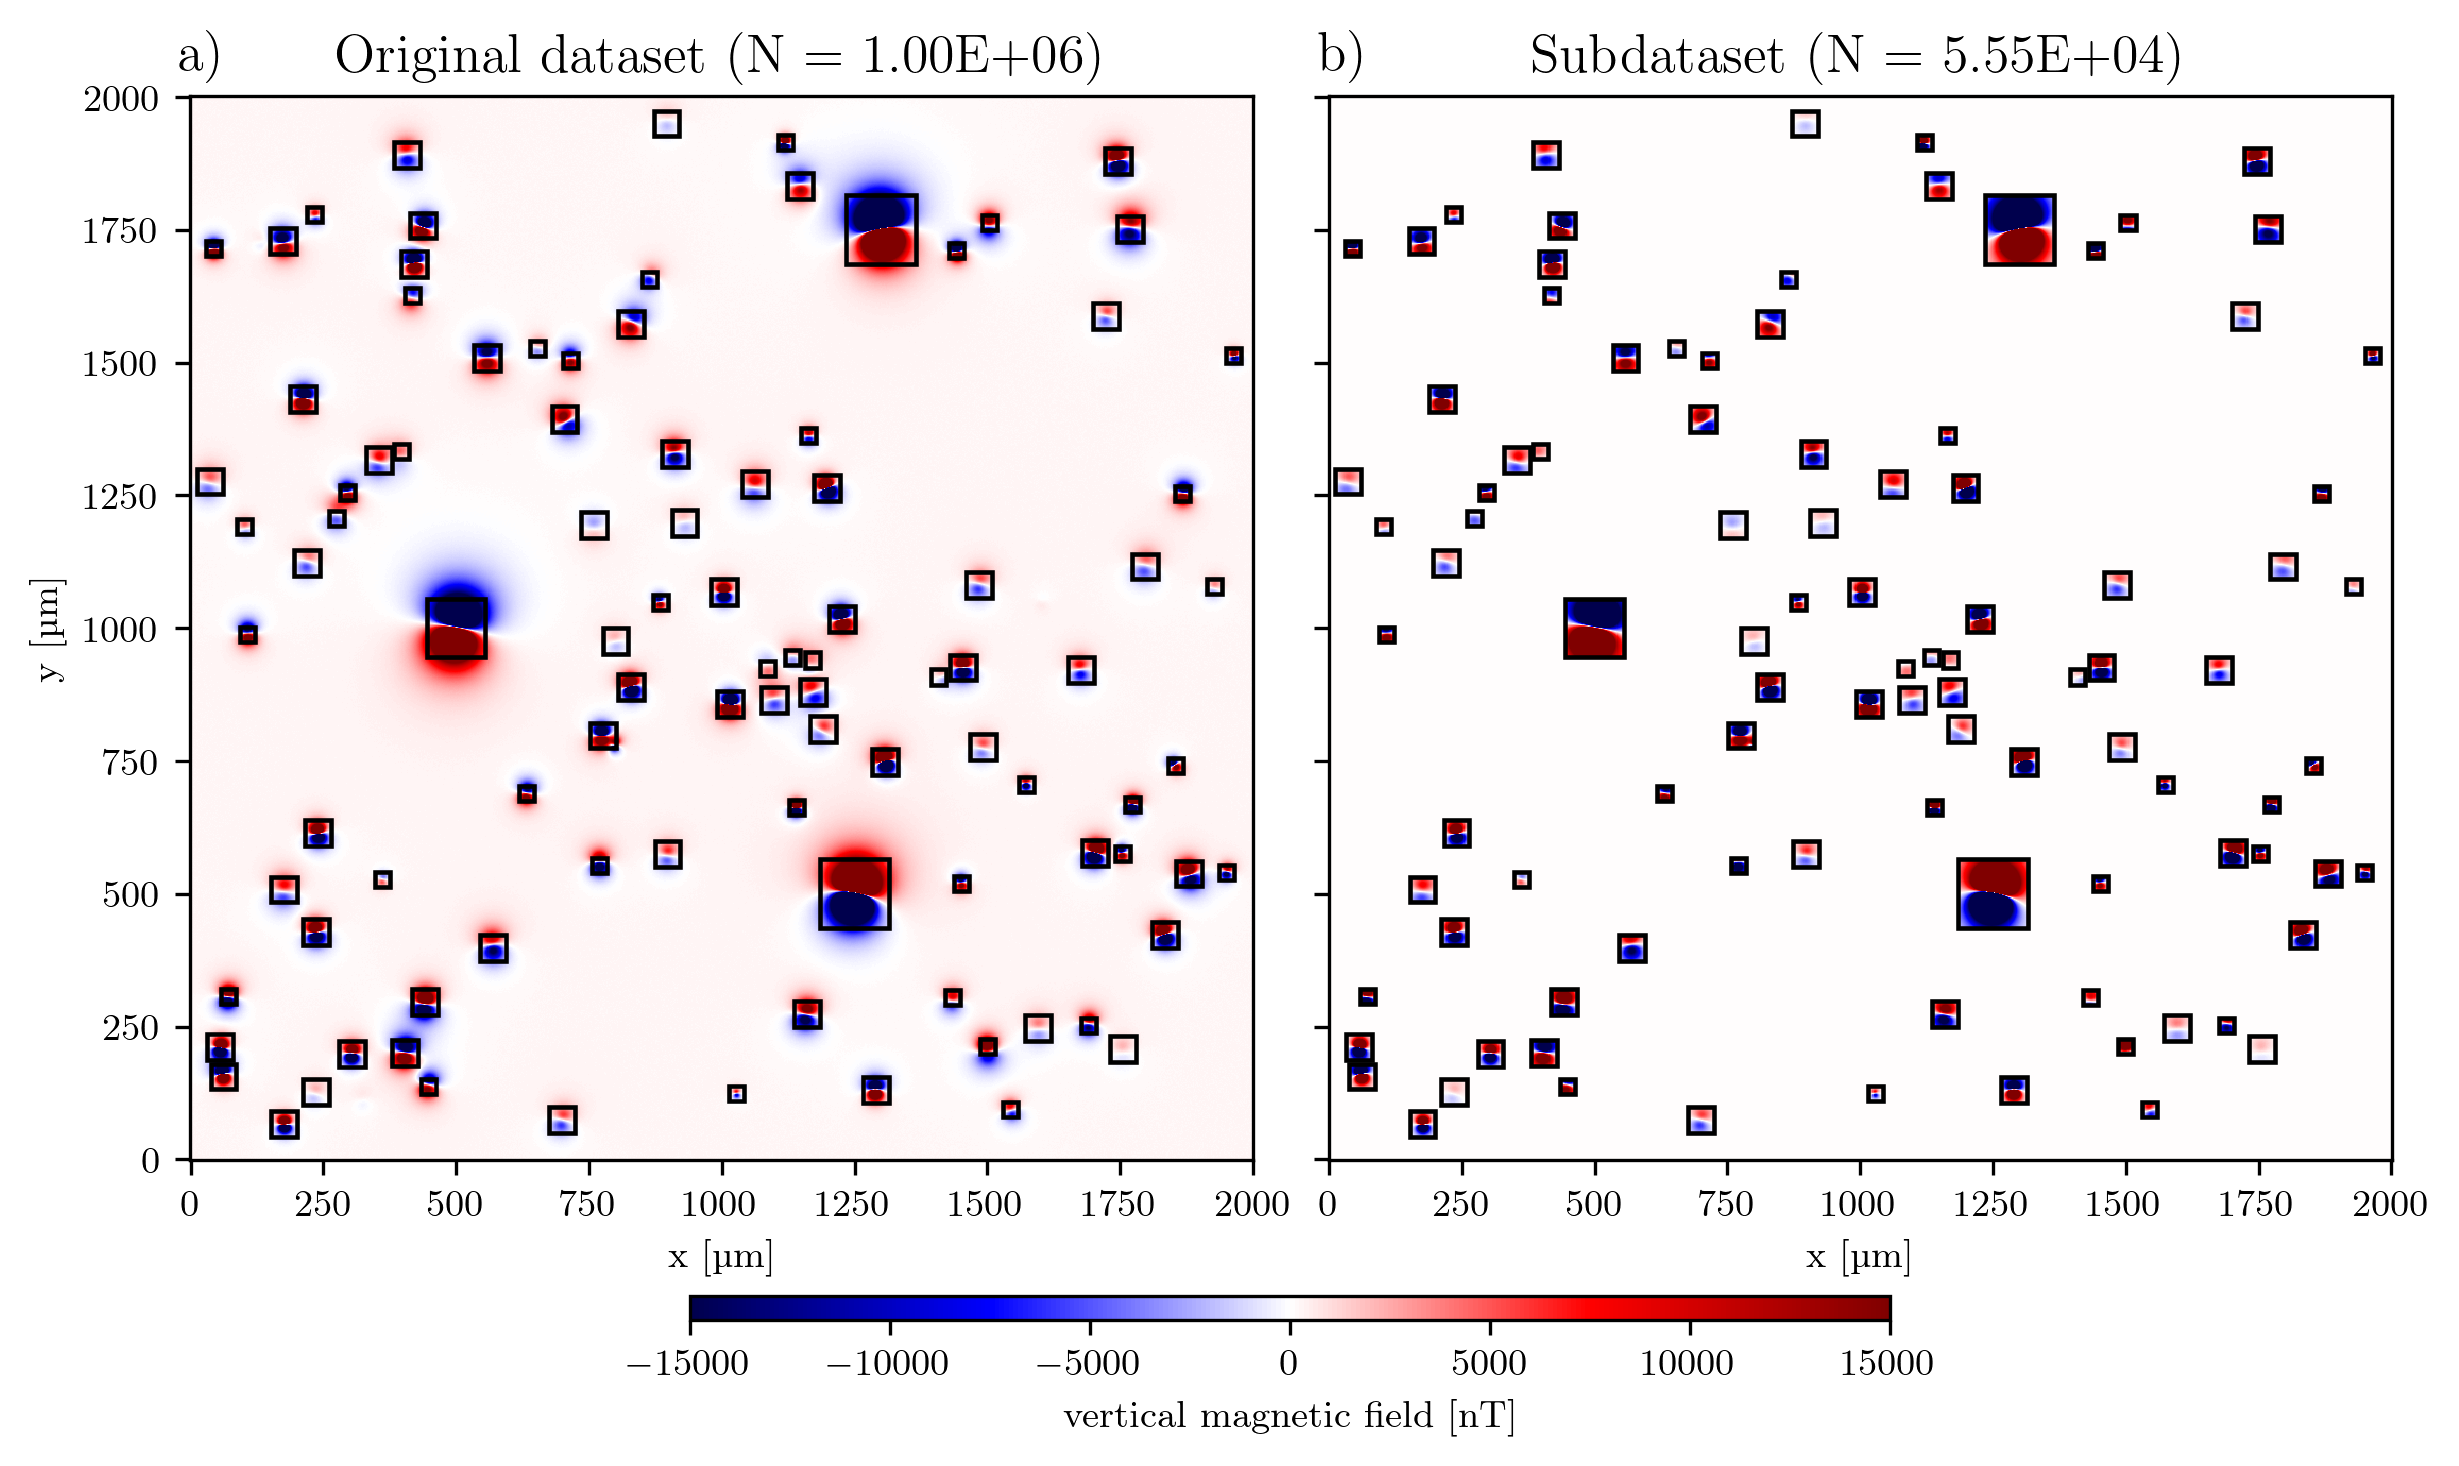
\includegraphics[width=1\linewidth]{figures/methodology.png}
  \caption{
    Tackling computational challenges in magnetic microscopy with extensive datasets.
    a) Complete synthetic dataset featuring all N observation points including areas lacking relevant information.
    b) Streamlining data through pre-selected windows reduces the dataset size for inversion, ensuring efficiency without compromising final results.
      }
  \label{methodology}
\end{figure}

%%%%%%%%%%%%%%%%%%%%%%%%%%%%%%%%%%%%%%%%%%%%%%%%%%%%%%%%%%%%%%%%%%%%%%%%%%%%%%%
